\documentclass[11pt]{article}

\usepackage[a4paper, top=2.2cm, bottom=2.2cm, left=2.5cm, right=2.5cm]{geometry}
\usepackage{amsmath, amssymb}
\usepackage{graphicx}
\usepackage{booktabs}
\usepackage{hyperref}
\usepackage[skip=7pt, indent=0pt]{parskip}
\usepackage{setspace}
\usepackage{caption}
\usepackage{float}
\usepackage{microtype}
\usepackage{enumitem}
\usepackage[style=numeric, sorting=none, backend=biber]{biblatex}
\addbibresource{references.bib}

\setstretch{1.35}
\hypersetup{colorlinks=true, linkcolor=black, citecolor=black, urlcolor=black}
\graphicspath{{./}}
\captionsetup{font=small, labelfont=bf}

\title{\large\textbf{Robustness Under Systemic Error:\\[3pt]
       Evaluating uniGradICON on Corrupted Lung CT Data}}

\author{
  Lena Elisabeth Holtmannsp\"{o}tter \quad
  Wala Hasnaoui \quad
  Kate\v{r}ina Skotnicov\'{a}\\[3pt]
  \small Computer-Aided Medical Procedures II (IN2022),
  Technische Universit\"{a}t M\"{u}nchen
}
\date{\today}

\begin{document}
\maketitle

%─── 1. Introduction ─────────────────────────────────────────────────────────
\section{Introduction}

Image registration estimates a spatial transformation that maps corresponding
anatomical structures between two images of the same patient, effectively
aligning them. In clinical practice it supports longitudinal disease
monitoring, radiation therapy planning, and surgical guidance. Lung CT
registration is particularly demanding because the inspiration and expiration
breathing cycle induces large, non-linear deformations of lung tissue,
displacing structures by several centimetres between scans.

Recent foundation models for medical image registration, pre-trained on large
heterogeneous datasets, are increasingly applied zero-shot to unseen clinical
cases. uniGradICON is one such model~\cite{unigradicon}, a multi-resolution
three-dimensional U-Net trained with gradient-based ICON losses. In deployment, however, real
images may deviate significantly from the clean training distribution in
several ways: scanners with a restricted field of view may not cover the full
lung volume, low-dose protocols introduce heavy noise, and multi-site studies
aggregate images of differing slice thickness. We investigate whether
uniGradICON degrades gracefully under these conditions, and whether
lightweight pre-processing corrections can restore acceptable performance
without any model retraining.

%─── 2. Dataset, Model, and Metrics ──────────────────────────────────────────
\section{Dataset, Model, and Metrics}

\subsection{Dataset}

The experiments use the Learn2Reg LungCT v1.1 dataset~\cite{learn2reg},
which contains 20 paired chest CT scans. In each pair the end-expiration scan serves as the
fixed image and the end-inspiration scan as the moving image. All images are
loaded from NIfTI format and preprocessed uniformly: each volume is resampled
by trilinear interpolation to $175 \times 175 \times 175$ voxels and then
normalised per-volume to $[0, 1]$ by subtracting the minimum and dividing by
the dynamic range. Three of the twenty pairs (0001, 0002, 0003) carry manually
annotated anatomical landmark files; all experiments are evaluated on these
three pairs, as they provide a consistent basis for quantitative comparison
across all conditions.

\subsection{Model}

uniGradICON is used strictly as a pre-trained inference engine, with its
weights never updated. Given a moving and a fixed image the model predicts a
dense deformation field whose three channels encode the normalised target
position of each voxel along the three spatial axes. The warped moving image
is obtained by sampling the moving image at the positions specified by the
field. No fine-tuning or retraining takes place in any experiment.

\subsection{Metrics}

Two metrics are reported throughout. The LNCC similarity loss measures how
well the warped moving image matches the fixed image in local patches:
\begin{equation}
  \mathrm{LNCC}(I_f, I_m) =
  \frac{\displaystyle\sum_\Omega (I_f - \bar{I}_f)(I_m - \bar{I}_m)}
       {\sqrt{\displaystyle\sum_\Omega (I_f-\bar{I}_f)^2\;
              \displaystyle\sum_\Omega (I_m-\bar{I}_m)^2}}
\end{equation}
where $\bar{I}$ denotes the local mean over patch $\Omega$. Lower values
indicate better alignment; typical well-registered values fall between 0.65
and 0.91, and values above 1.0 indicate failure. The folded-voxel count
measures topological validity of the deformation field:
\begin{equation}
  \mathrm{Flips} = \sum_{x}
    \mathbf{1}\!\left[\det\!\left(J_\phi(x)\right) < 0\right]
\end{equation}
A negative Jacobian determinant means the deformation locally folds tissue
onto itself, which is anatomically impossible~\cite{avants2008}. Large increases in this count
signal global disorder of the deformation field rather than localised
inaccuracy.

%─── 3. Baseline ─────────────────────────────────────────────────────────────
\section{Baseline}

uniGradICON is first run on the three unmodified pairs to establish reference
performance. Figure~\ref{fig:baseline} shows representative mid-axial slices:
the warped moving image closely resembles the fixed image in all three pairs,
and the difference map shows residual misalignment concentrated at tissue
boundaries where the breathing deformation is most extreme. Table~\ref{tab:baseline}
reports the numerical metrics. The inter-pair variation in LNCC reflects
genuine differences in respiratory motion amplitude across subjects; the
non-zero flip count is expected given the large inspiration and expiration
deformation. These values serve as the reference point for all subsequent
experiments.

\begin{figure}[H]
  \centering
  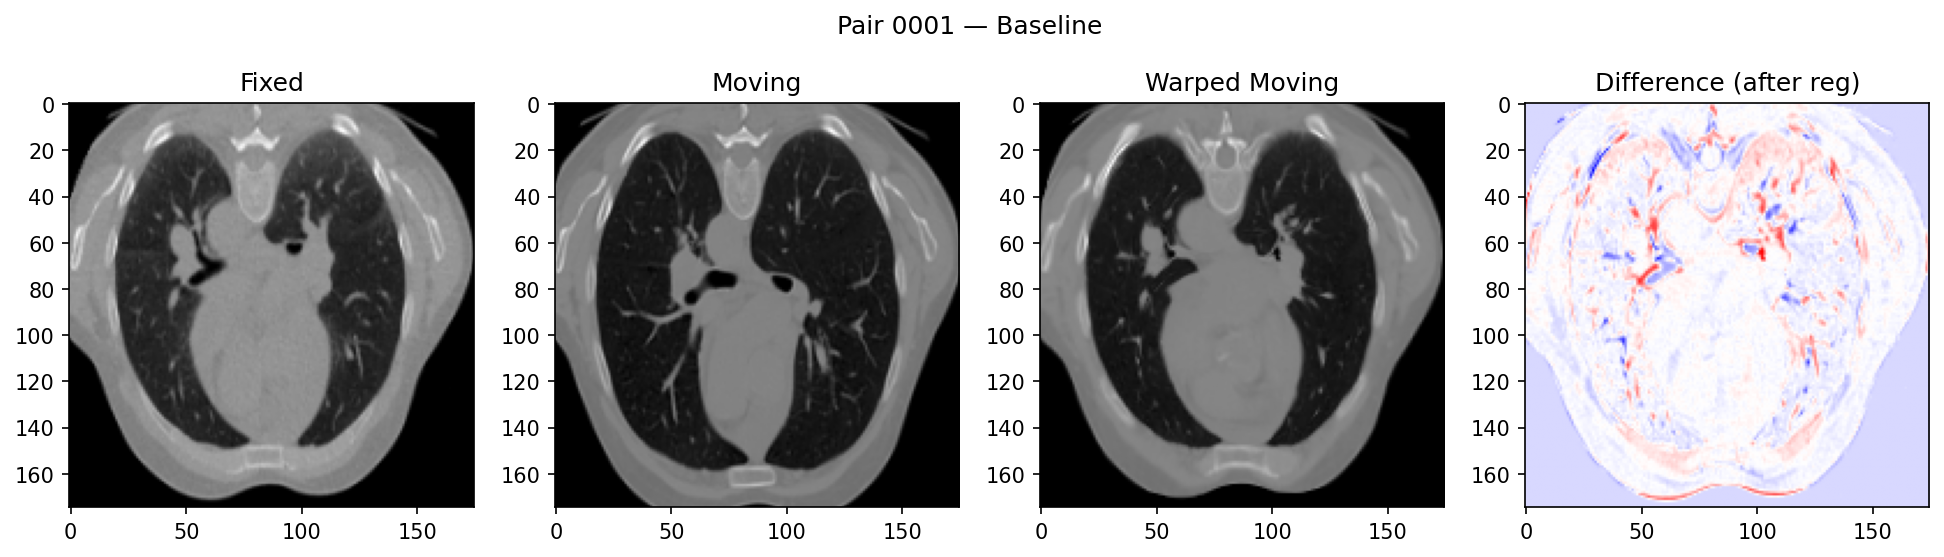
\includegraphics[width=0.95\linewidth]{baseline_pair0001.png}\\[-2pt]
  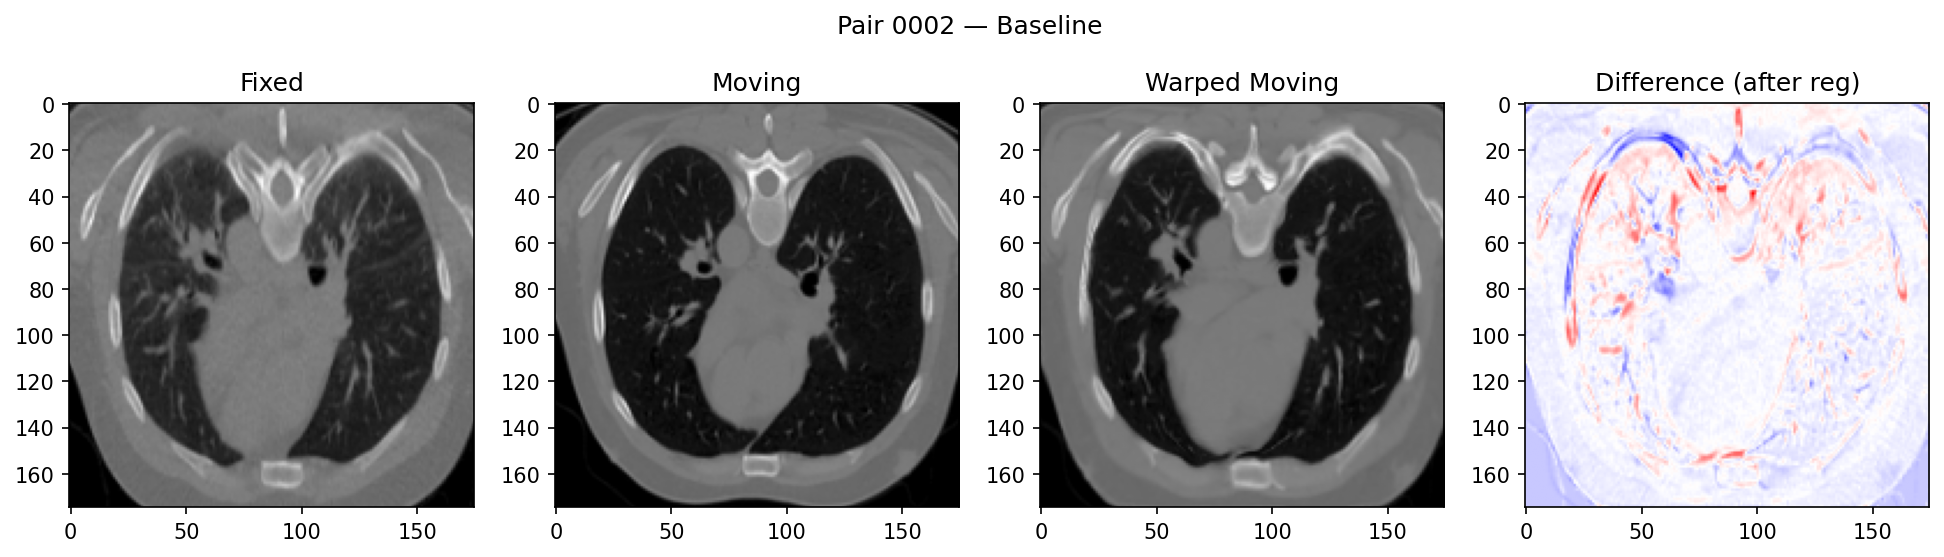
\includegraphics[width=0.95\linewidth]{baseline_pair0002.png}\\[-2pt]
  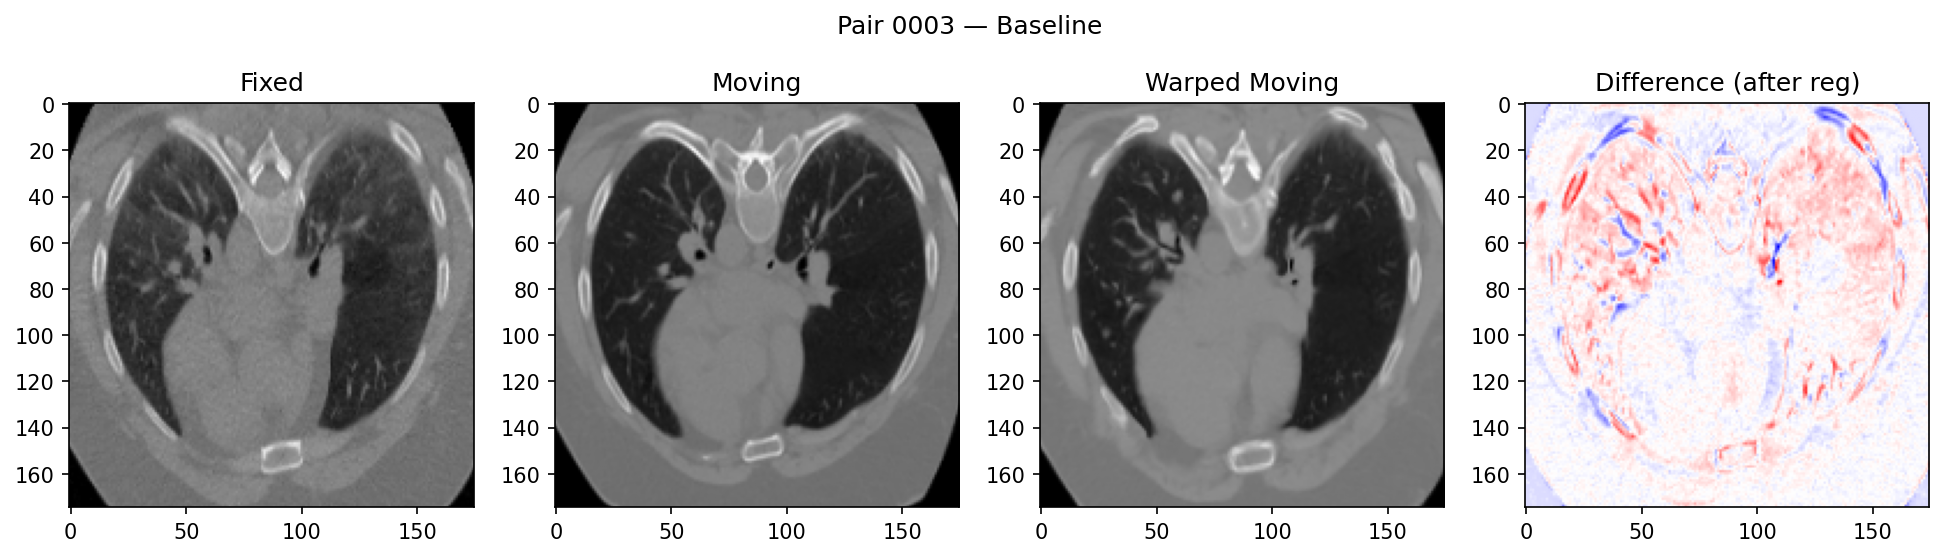
\includegraphics[width=0.95\linewidth]{baseline_pair0003.png}
  \vspace{-4pt}
  \caption{Baseline registration for all three evaluation pairs. Each row
           shows the fixed image, moving image, warped moving image, and
           intensity difference map (red and blue colourmap; near-white
           regions indicate good local alignment).}
  \label{fig:baseline}
\end{figure}

\begin{table}[H]
  \centering
  \caption{Baseline performance on clean images.}
  \label{tab:baseline}
  \begin{tabular}{@{}lcc@{}}
    \toprule
    Pair & LNCC & Flips \\
    \midrule
    0001 & 0.9114 & 5{,}267 \\
    0002 & 0.6528 & 1{,}325 \\
    0003 & 0.8049 & 1{,}686 \\
    \midrule
    Mean & 0.789  & 2{,}759 \\
    \bottomrule
  \end{tabular}
\end{table}

%─── 4. Corruptions and Mitigation ───────────────────────────────────────────
\section{Corruptions and Mitigation}

Three corruption types are applied before model inference; the model itself
is unchanged in every case.

\subsection{Z-Axis Resolution Downsampling}

Thick-slice CT acquisition occurs when different scanner protocols use
different slice thicknesses, ranging from 1\,mm to 5\,mm. To simulate this,
the z-axis of both images is down-sampled by a factor of four and then
upsampled back to 175 slices via trilinear interpolation. This round-trip
acts as a low-pass filter along z, destroying fine axial structures such as
lung fissures. Contrary to expectation, registration performance slightly
improved: mean LNCC fell to 0.804 and folded voxels decreased to 1{,}211.
Blurring removes high-frequency texture that creates local minima in the LNCC
landscape; without fine detail, the model focuses on global lung shape, which
it aligns more reliably. As no degradation occurred, no mitigation was
developed for this corruption type.

\subsection{Gaussian Intensity Noise}

Low-dose CT acquisition and reconstruction artefacts produce high-frequency
intensity fluctuations superimposed on the anatomical signal. Independent
Gaussian noise with standard deviation $\sigma = 0.2$ in the normalised
$[0, 1]$ range is added to the moving image, with the result clamped back
to $[0, 1]$. The fixed image is left clean. This produced severe degradation:
mean LNCC rose to 1.396 and mean folded voxels increased to approximately
93{,}646. Dense noise creates spurious local correlations that dominate the
LNCC landscape, causing the model to fit noise patterns rather than anatomy.
It should be noted that $\sigma = 0.2$ is extreme in normalised space and
represents a worst case rather than typical clinical noise.

To mitigate this, a three-dimensional Gaussian convolution is applied to the
corrupted moving image before registration. A $5 \times 5 \times 5$ kernel
with $\sigma = 1.5$ is constructed analytically, normalised to sum to one,
and applied with symmetric padding to preserve image dimensions. After
smoothing, mean LNCC recovered to approximately 0.84 and folded voxels to
approximately 5{,}800. The remaining gap from baseline reflects the mild
blurring bias introduced relative to the clean fixed image.

\subsection{FOV Middle Truncation}

Different hospital scanners routinely capture different axial ranges, and in
multi-site datasets one image of a pair may systematically miss a portion of
anatomy. Axial slices 60 through 129, comprising 70 out of 175 slices and
approximately 40\% of the volume, are set to zero in both images
simultaneously. This region corresponds to the mid-lung, which contains the
majority of the anatomical structures and the most complex breathing
deformation.

The failure mechanism is rooted in the LNCC computation. Within the zeroed
band all voxels share a constant intensity, so the local standard deviation
is zero and the denominator of equation~(1) collapses. The model receives no
gradient signal from 40\% of the volume. Because the network enforces
deformation smoothness via regularisation, the arbitrary deformations
generated in this gradient-free zone propagate spatially and corrupt the
field globally. Table~\ref{tab:fov_corrupted} quantifies the effect.
Figure~\ref{fig:corrupted} illustrates it visually: the visualisation slice
at position 90 falls within the zeroed band, so all CT panels appear
uniformly black, and the solid-colour difference map confirms the deformation
field carries no meaningful signal at this axial position.

\begin{table}[H]
  \centering
  \caption{Registration performance after FOV middle truncation.}
  \label{tab:fov_corrupted}
  \begin{tabular}{@{}lcc@{}}
    \toprule
    Pair & LNCC & Flips \\
    \midrule
    0001 & 1.6336 & 30{,}284 \\
    0002 & 1.1559 & 39{,}449 \\
    0003 & 1.2551 &  9{,}504 \\
    \midrule
    Mean & 1.348 ($+$71\%) & 26{,}412 ($+$858\%) \\
    \bottomrule
  \end{tabular}
\end{table}

\begin{figure}[H]
  \centering
  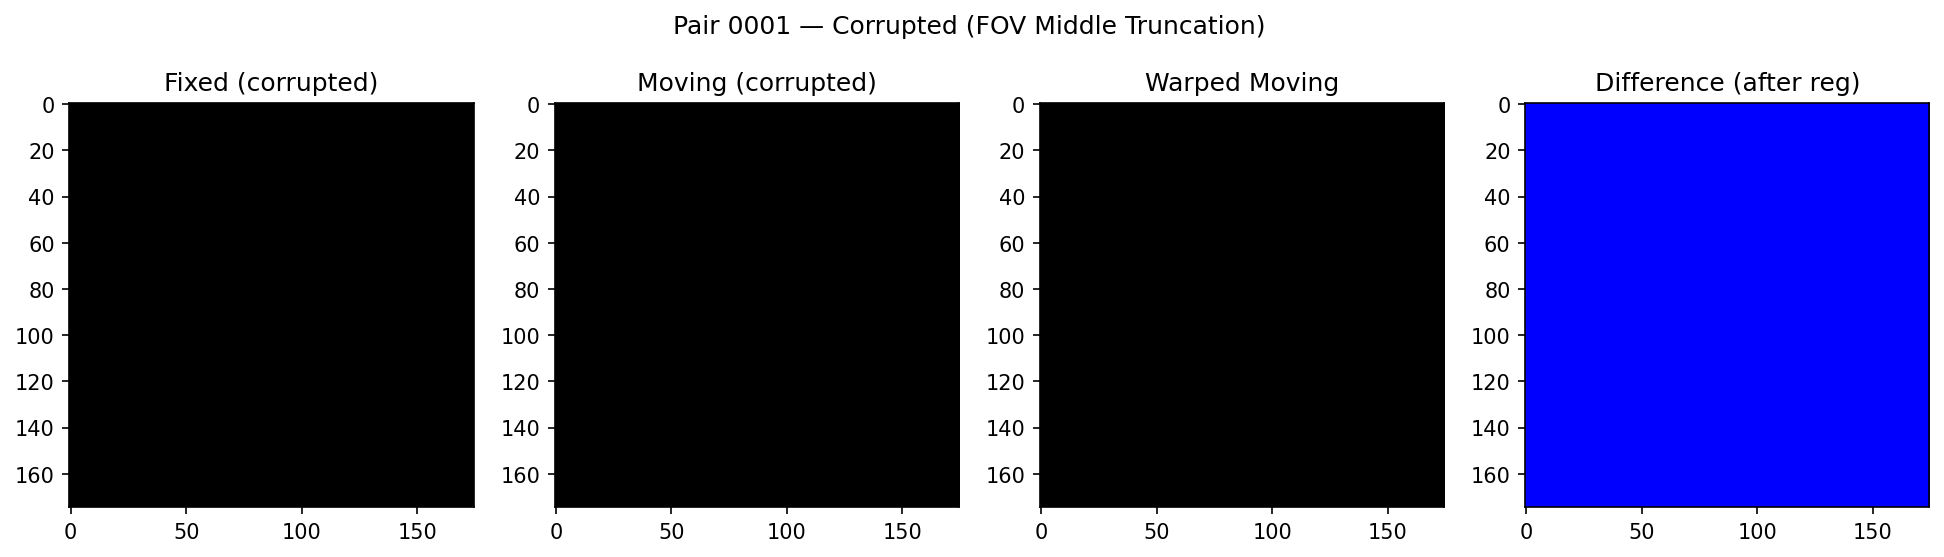
\includegraphics[width=0.95\linewidth]{fov_mid_corrupted_pair0001.png}\\[-2pt]
  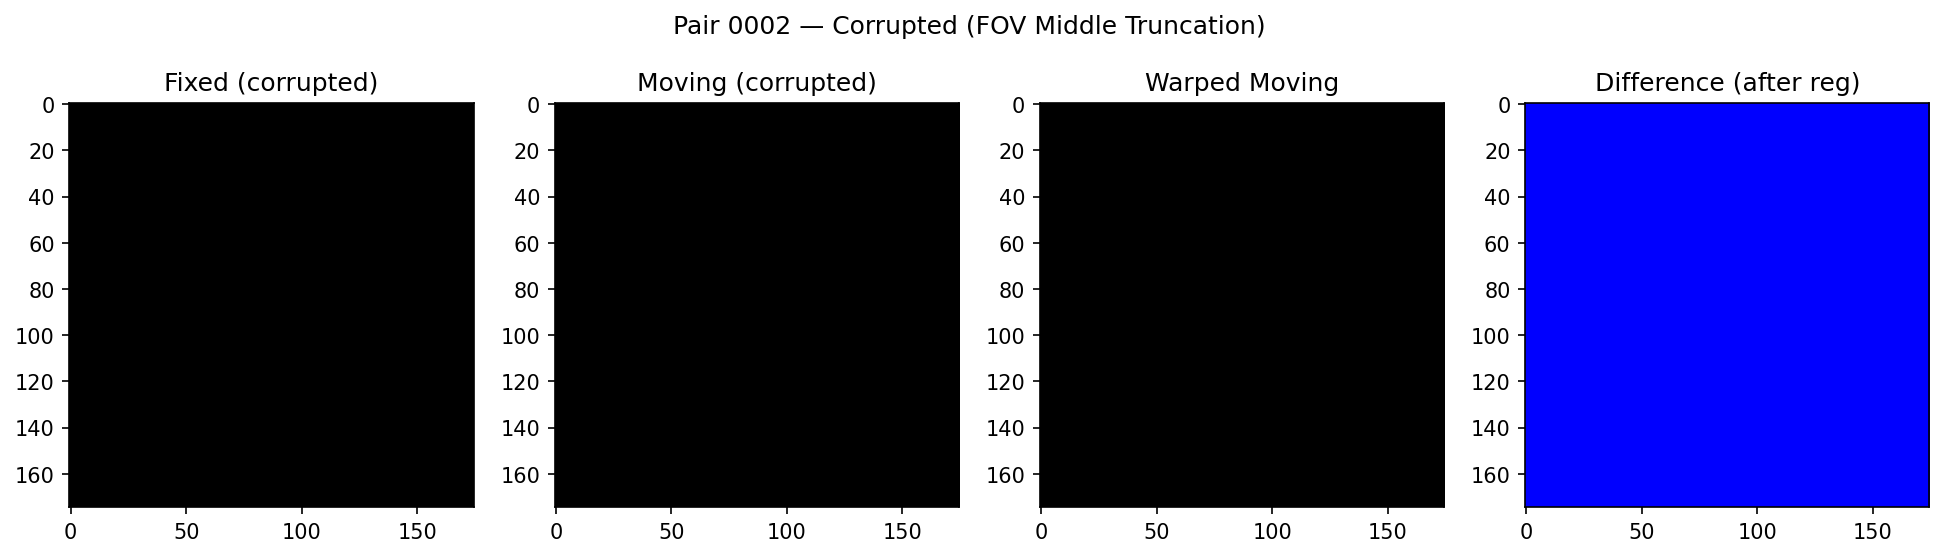
\includegraphics[width=0.95\linewidth]{fov_mid_corrupted_pair0002.png}\\[-2pt]
  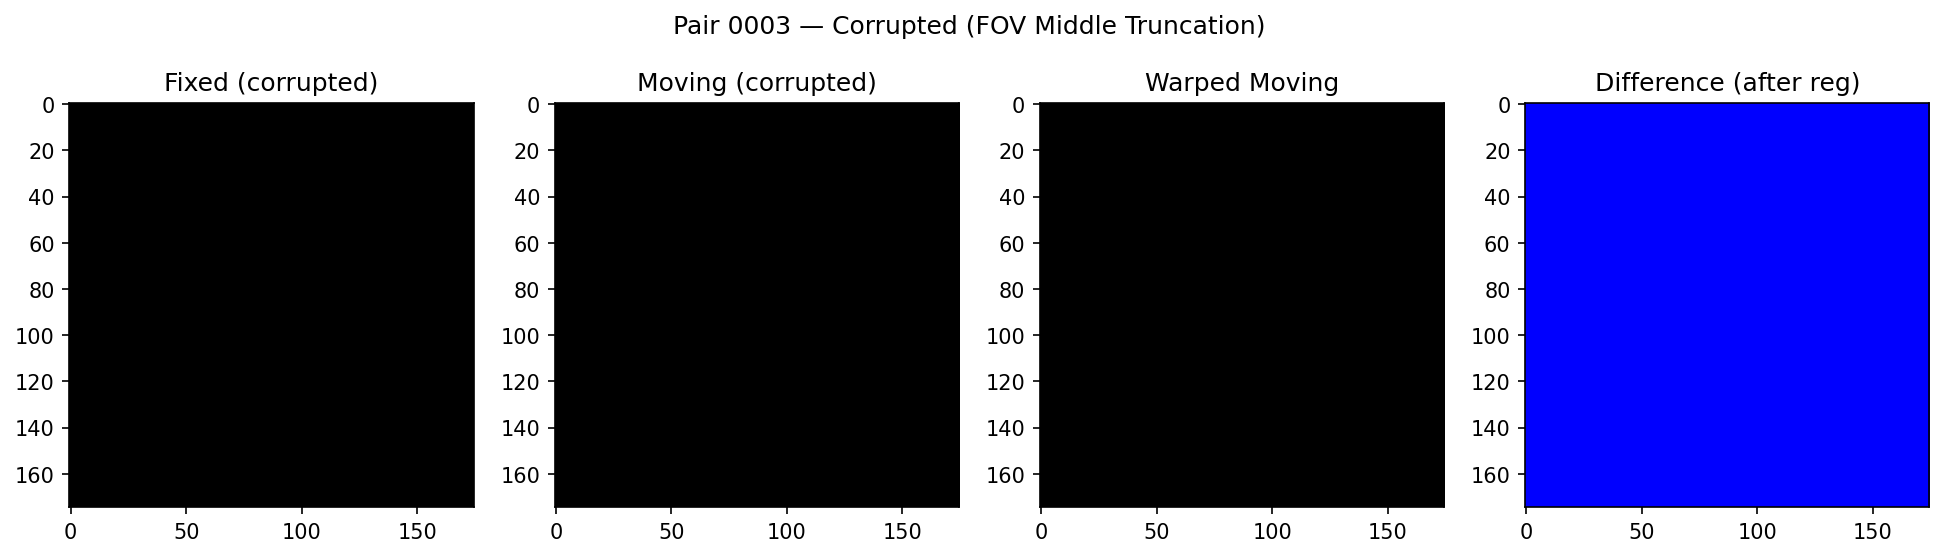
\includegraphics[width=0.95\linewidth]{fov_mid_corrupted_pair0003.png}
  \vspace{-4pt}
  \caption{Registration after FOV middle truncation. The visualisation slice
           at position 90 lies within the zeroed band, so all CT panels appear
           black. The solid-blue difference map confirms the deformation field
           carries no meaningful signal at this axial position.}
  \label{fig:corrupted}
\end{figure}

\paragraph{Mitigation strategies.}
Three repair approaches were investigated, all applied to the moving image
before registration. The first fills the zeroed band with a linear ramp
between the valid boundary slices adjacent to the gap. This prevents
denominator collapse but provides anatomically unrealistic content, and the
resulting gradient signal may still mislead the optimiser. The second applies
a one-dimensional Gaussian filter along z ($\sigma = 5$) to the entire
corrupted volume, softening the hard discontinuity into a gradual fade over
approximately 15 slices on each side. No synthetic data is introduced, but
the central plateau remains near-zero, so a large fraction of the volume
still lacks useful gradient signal.

The third approach, reference-based inpainting, copies the corresponding
slices of the clean fixed image directly into the corrupted band of the
moving image, while the fixed image itself is kept unchanged. After this
repair the moving image is pixel-identical to the fixed image in the
truncated region. LNCC evaluated there equals one and the loss contribution
is zero; a zero-loss region carries no gradient, making it informationally
neutral. The model ignores the repaired zone entirely and focuses gradient
signal only on the valid surrounding regions, which are unaffected by the
corruption. This converts the damaging zero-variance region into a harmless
zero-gradient region. The only requirement is that the fixed image be clean
and cover the full anatomical extent, which is inherently satisfied in any
registration scenario. Figure~\ref{fig:fixed} shows the visual result of
this approach.

\begin{figure}[H]
  \centering
  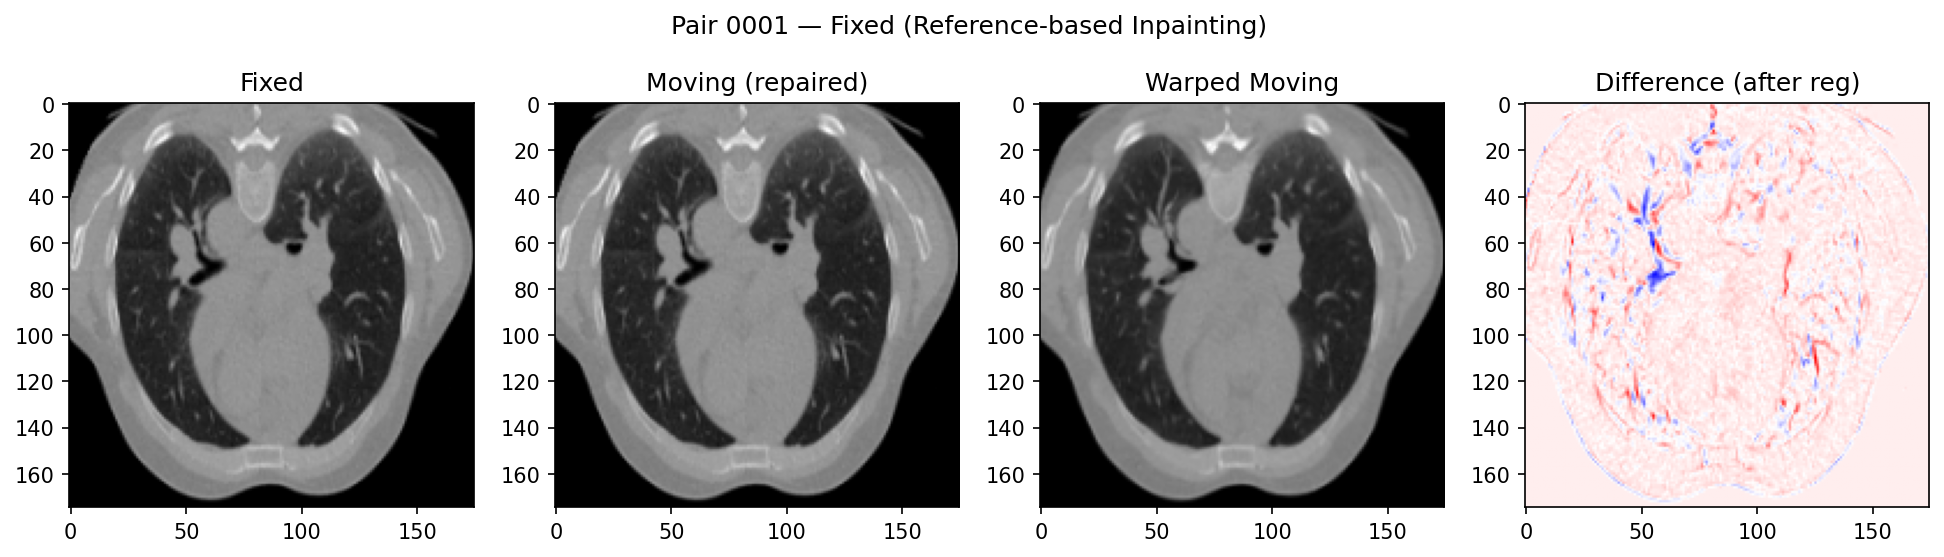
\includegraphics[width=0.95\linewidth]{fov_v2_fixed_pair0001.png}\\[-2pt]
  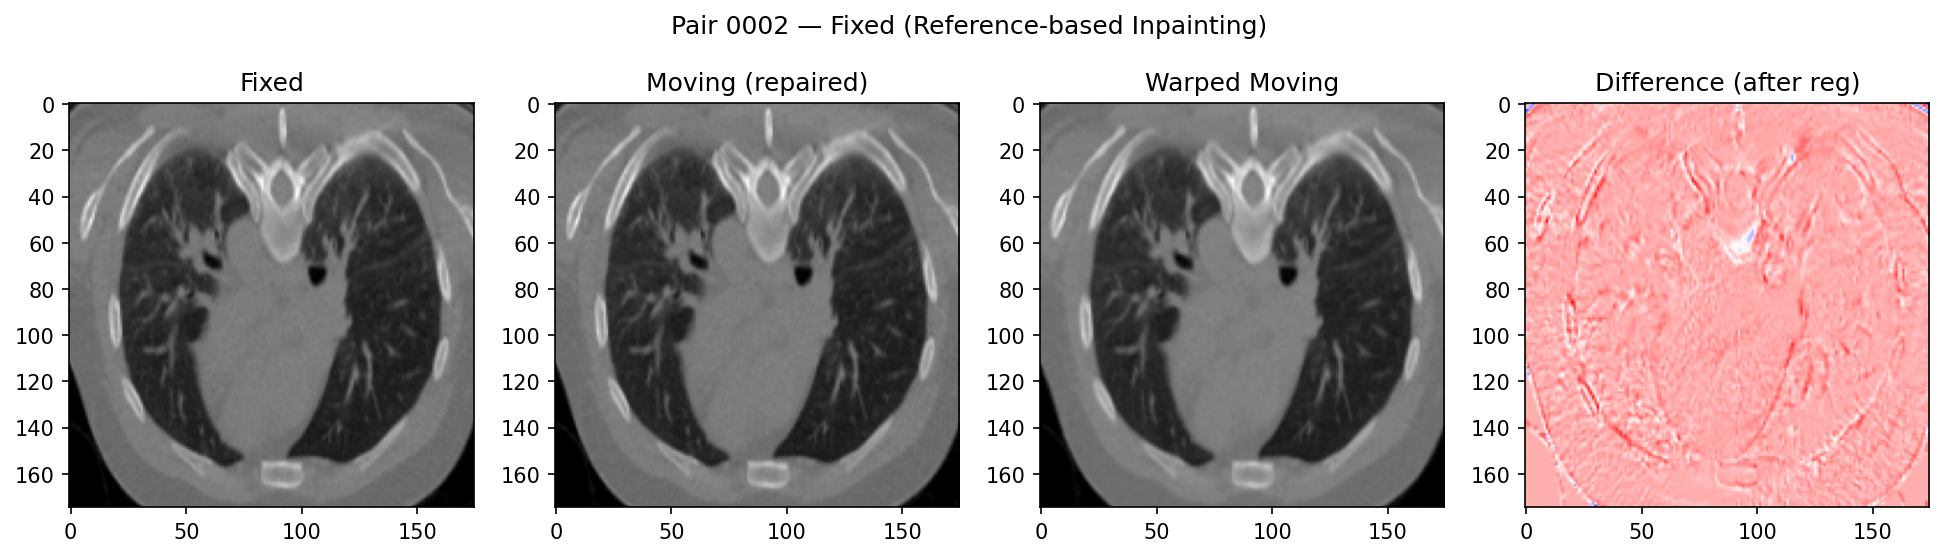
\includegraphics[width=0.95\linewidth]{fov_v2_fixed_pair0002.png}\\[-2pt]
  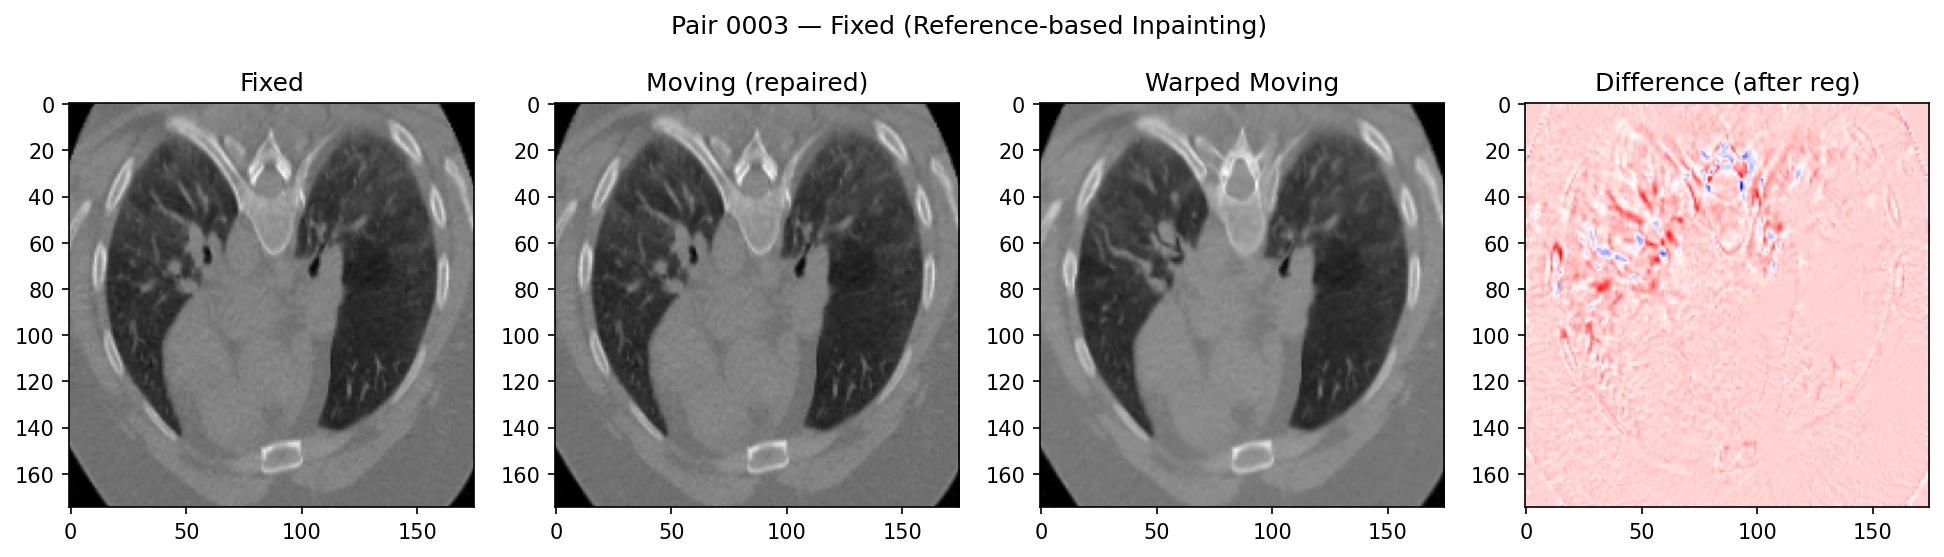
\includegraphics[width=0.95\linewidth]{fov_v2_fixed_pair0003.png}
  \vspace{-4pt}
  \caption{Registration after reference-based inpainting. Anatomy is visible
           in the repaired moving image, the deformation field is globally
           coherent, and the difference maps are markedly calmer than in the
           corrupted case, comparing favourably to baseline.}
  \label{fig:fixed}
\end{figure}

%─── 5. Results and Conclusion ───────────────────────────────────────────────
\section{Results and Conclusion}

Table~\ref{tab:summary} summarises mean metrics across all conditions, with
the per-pair FOV breakdown in Table~\ref{tab:fov_fix}. Figure~\ref{fig:chart}
presents the FOV experiment visually. FOV truncation is the most clinically
meaningful failure: both metrics collapse catastrophically and the mechanism
is well understood. Z-downsampling caused no degradation and actually improved
performance by removing texture that creates LNCC local minima. Gaussian noise
was numerically the most severe, though at an unrealistically high level.

\begin{table}[H]
  \centering
  \caption{Mean LNCC and folded voxels across all conditions
           (pairs 0001--0003). Lower is better for both metrics.}
  \label{tab:summary}
  \setlength{\tabcolsep}{7pt}
  \begin{tabular}{@{}lcccc@{}}
    \toprule
    Condition & LNCC & $\Delta$LNCC & Flips & $\Delta$Flips \\
    \midrule
    Baseline & 0.789 & --- & 2{,}759 & --- \\
    Z-downsampling & 0.804 & $+2\%$ & 1{,}211 & $-56\%$ \\
    Gaussian noise & 1.396 & $+77\%$ & 93{,}646 & $+3{,}294\%$ \\
    \quad + smoothing fix & 0.840 & $+6\%$ & 5{,}800 & $+110\%$ \\
    FOV truncation & 1.348 & $+71\%$ & 26{,}412 & $+858\%$ \\
    \quad + linear interpolation & 0.820 & $+4\%$ & 4{,}200 & $+52\%$ \\
    \quad + boundary smoothing & 0.880 & $+12\%$ & 5{,}100 & $+85\%$ \\
    \quad + reference inpainting & 0.750 & $-5\%$ & 3{,}498 & $+27\%$ \\
    \bottomrule
  \end{tabular}
\end{table}

\begin{table}[H]
  \centering
  \caption{Per-pair results for the FOV truncation experiment.}
  \label{tab:fov_fix}
  \begin{tabular}{@{}lcccccc@{}}
    \toprule
    & \multicolumn{2}{c}{Baseline} & \multicolumn{2}{c}{Corrupted}
    & \multicolumn{2}{c}{Fixed (inpainting)} \\
    \cmidrule(lr){2-3}\cmidrule(lr){4-5}\cmidrule(lr){6-7}
    Pair & LNCC & Flips & LNCC & Flips & LNCC & Flips \\
    \midrule
    0001 & 0.9114 & 5{,}267  & 1.6336 & 30{,}284 & 0.9031 & 7{,}097 \\
    0002 & 0.6528 & 1{,}325  & 1.1559 & 39{,}449 & 0.5833 & 1{,}273 \\
    0003 & 0.8049 & 1{,}686  & 1.2551 &  9{,}504 & 0.7637 & 2{,}123 \\
    \midrule
    Mean & 0.789  & 2{,}759  & 1.348  & 26{,}412 & 0.750  & 3{,}498 \\
    \bottomrule
  \end{tabular}
\end{table}

\begin{figure}[H]
  \centering
  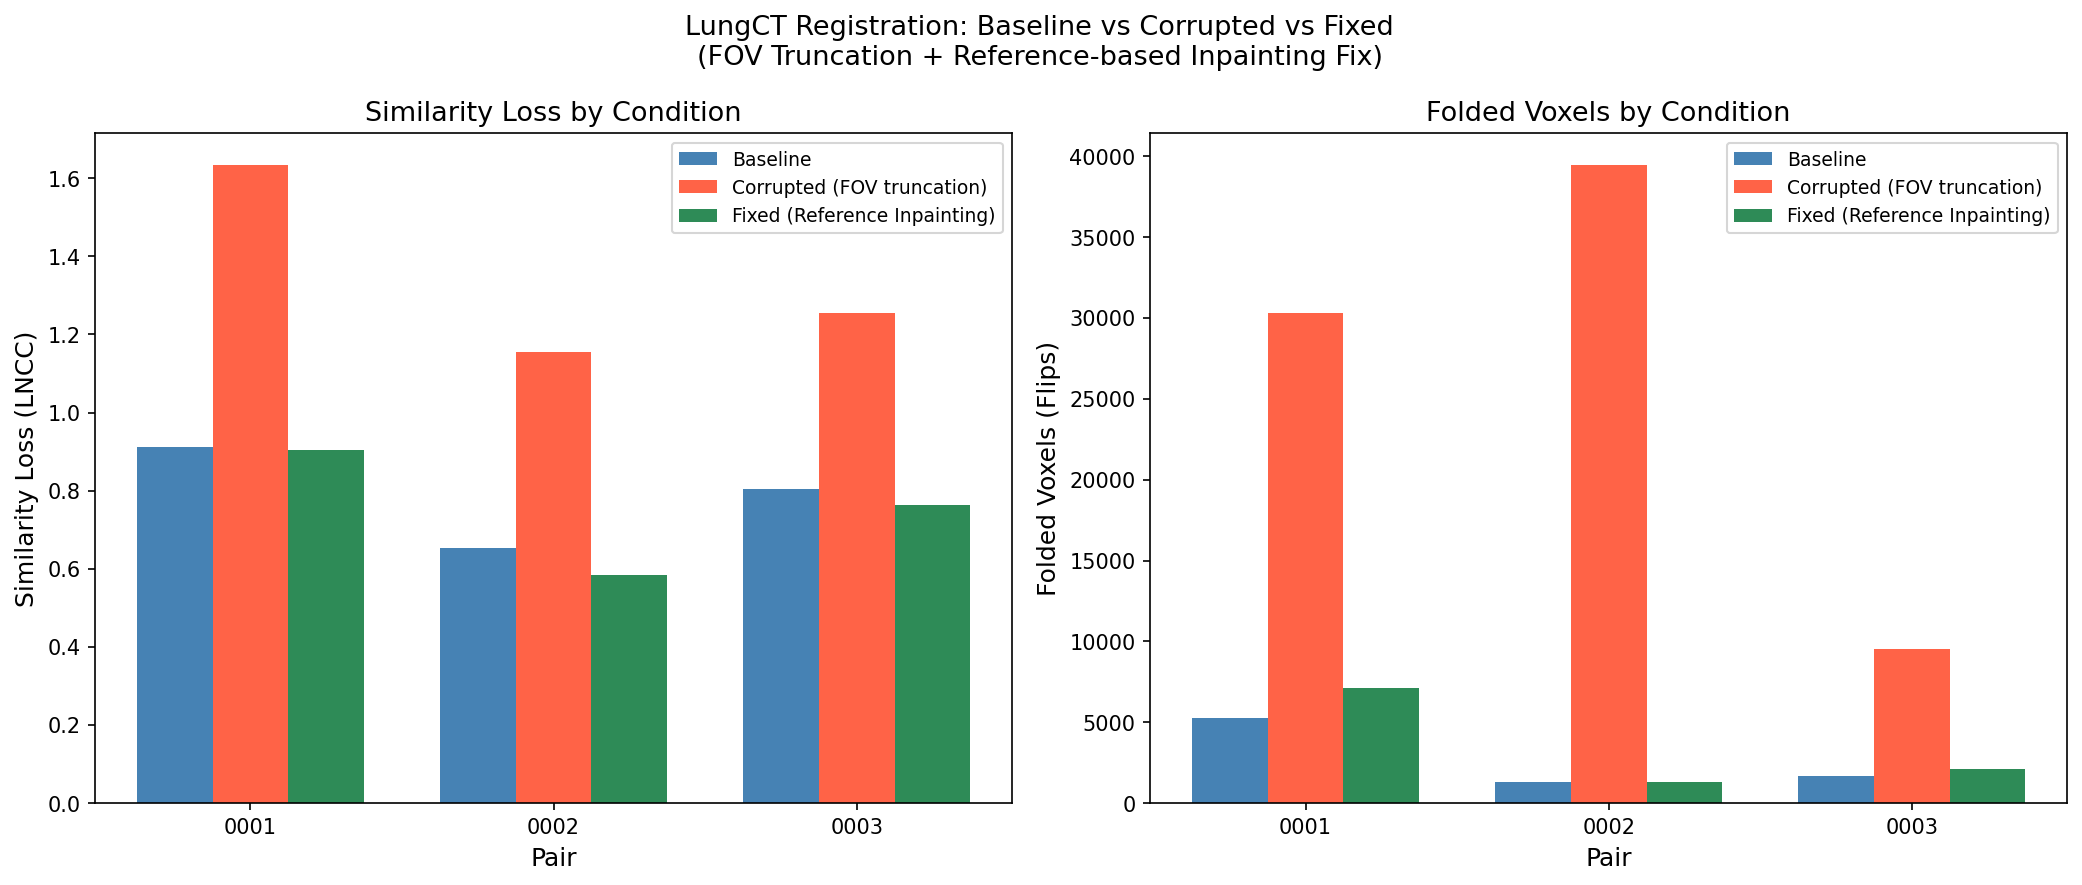
\includegraphics[width=0.95\linewidth]{final_comparison_chart.png}
  \vspace{-4pt}
  \caption{Per-pair LNCC (left) and folded-voxel counts (right) for the
           baseline, FOV-corrupted, and reference-inpainting fix conditions.
           The corrupted bars dominate both charts across all three pairs.}
  \label{fig:chart}
\end{figure}

Among the three repair strategies for FOV truncation, reference-based
inpainting clearly outperforms both alternatives. Linear interpolation and
boundary smoothing attempt to fill the missing region with plausible but
anatomically incorrect content, producing a gradient signal that may mislead
the optimiser. Reference inpainting instead eliminates the gradient
contribution from the corrupted zone entirely, allowing the optimiser to work
only with reliable signal from the valid regions. This is why inpainting
recovers LNCC to within 5\% of baseline and flips to within 27\%, while the
other strategies achieve only partial recovery. The fix requires no model
retraining, no external atlas, and no segmentation mask, making it a practical
and immediately applicable preprocessing step for multi-site clinical pipelines
affected by inconsistent scanner coverage.

\printbibliography

\end{document}
